\documentclass[12pt]{article}
\usepackage{amsmath}
\usepackage{amssymb}
\usepackage{blindtext}
\usepackage{geometry}
\geometry{a5paper, margin=0.2in, bottom=0.5in}
\usepackage[english, russian]{babel}
\usepackage[utf8]{inputenc}
\usepackage{graphicx}
\usepackage{caption}
\usepackage{subcaption}
\usepackage{float}
\usepackage{comment}

\usepackage{listings}

\graphicspath{ {./images/} }

\title{Лабораторная работа №2:\\ \large{Численные методы вычисления интегралов\\Индивидуальная часть}}
\author{Ушаков Роман}
\date{10.04.2026}

\begin{document}
\maketitle

20 вариант: \(f(x)=\cos{2x}, [0, \frac{\pi}{2}]\)
\vspace{0.2cm}\\
Разбиение отрезка везде предполагается равномерным.
\begin{comment}
{\largeПлан работы}:
\begin{enumerate}
  \item \textbf{Составьте} интегральную сумму для интеграла Римана данной функции по данному промежутку.
  \item \textbf{Вычислите} интеграл через предел интегральных сумм.
  \item \textbf{Докажите}, что соответствующий интеграл существует.
  \item \textbf{Проверьте} вычисление при помощи формулы Ньютона–Лейбница.
  \item Напишите программу, \textbf{вычисляющую} и \textbf{отрисовывающую} интегральные суммы для данной функции на данном отрезке. Входные данные для программы: число точек разбиения, способ выбора оснащения (левые, правые, средние, трапеция).
  \item \textbf{Найдите} погрешность оценки, сравните ее с теоретической погрешностью.
  \item \textbf{Выведите} формулы для оценки погрешности.
\end{enumerate}
\end{comment}

\subsection*{Часть 1. Вычисление интеграла}

1. \textbf{Интегральная сумма}

Дан интеграл:
\[\int\limits_0^{\pi/2} \cos{2x} \, dx\]

Для нахождения суммы для интеграла Римана на \([a, b]\) воспользуемся формулой правых прямоугольников:
\[\lim\limits_{n\to\infty}\frac{b-a}{n}\sum^{n-1}_{i=0}{f(x^i)}\]

В нашем случае:
\[I=\lim\limits_{n\to\infty}\frac{\pi/2}{n}\sum^{n-1}_{k=0}{\cos{(2k \cdot \frac{\pi/2}{n})}}\]

\vspace{0.2cm}

\newpage

2. \textbf{Вычисление суммы}

Для вычисления суммы косинусов, воспользуемся данной формулой:
\[\sum_{k=0}^{n-1} \cos(k \cdot \alpha) = \frac{\sin(n \alpha /2)}{\sin(\alpha / 2)} \cdot \cos(\frac{(n-1)\alpha}{2}), \text{ при } \sin(\alpha/2) \neq 0.\]

Подставляем(\(\alpha = \frac{\pi}{n}\)):
\[I=\lim\limits_{n\to\infty} (\frac{\pi/2}{n} \cdot \frac{\sin(\pi/2)}{\sin(\frac{\pi}{2n})} \cdot \sin(\frac{\pi}{2n}))=\lim\limits_{n\to\infty}\frac{\pi/2}{n}=0\]

\vspace{0.2cm}

3. \textbf{Проверка существования интеграла}

Данная функция \(\cos(2x)\) непрерывна на отрезке \([a, b]\), что является достаточным условием для существования интеграла.

\vspace{0.2cm}

4. \textbf{Проверка прямым интегрированием}

\[\int\limits_0^{\pi/2} \cos{2x} \, \left.dx=\frac{1}{2}\sin(2x)\right|_0^{\pi/2}=\frac{1}{2}\sin(\pi)-\frac{1}{2}\sin(0)=0.\]

\subsection*{Часть 2. Численное интегрирование}

Задание выполнено на языке программирования Python.
Для отрисовки графиков использовалась библиотека matplotlib.\\
Значение исходного определенного интеграла: \(I=0\).\\
Значение первой половины: \(I=0.5\)

\newpage

{\large Метод левых прямоугольников}\\
Вычисление ошибки: 
\(|R_n|\leq \max\limits_{x\in[a,b]}{|f'(x)|\frac{(b-a)^2}{2n}}\) \\

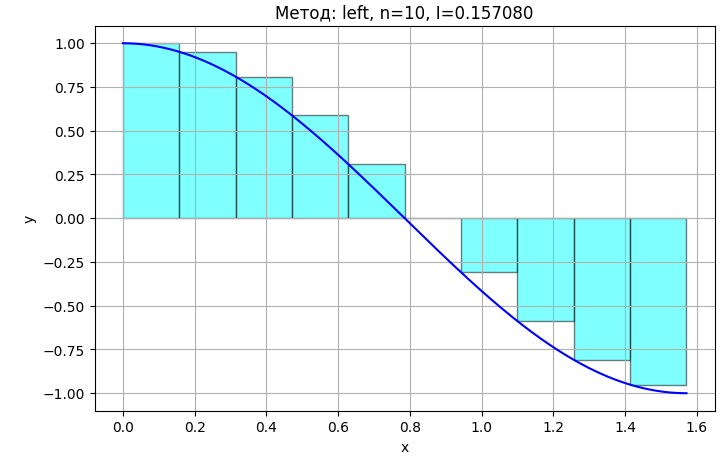
\includegraphics[width=0.6\linewidth]{left_n10.png}\\
\(n=10, R = 0.157080\) \\
\(|R_n|\leq \max\limits_{x\in[0,\pi/2]}{|-2\sin{2x}|\frac{(\pi/2)^2}{2n}}=
2\ \cdot\ \frac{(\pi/2)^2}{2n}=\frac{\pi^2}{4n}\) \\
\(|R_n|\leq \frac{\pi^2}{4n}=\frac{\pi^2}{4\cdot 10} \approx 0.246740\)\\
\(|R_n| \leq 0.246740\), \(|R-I|\approx0.157080\),\\
погрешность расчетов не превышает теоретическую.

\vspace{0.5cm}

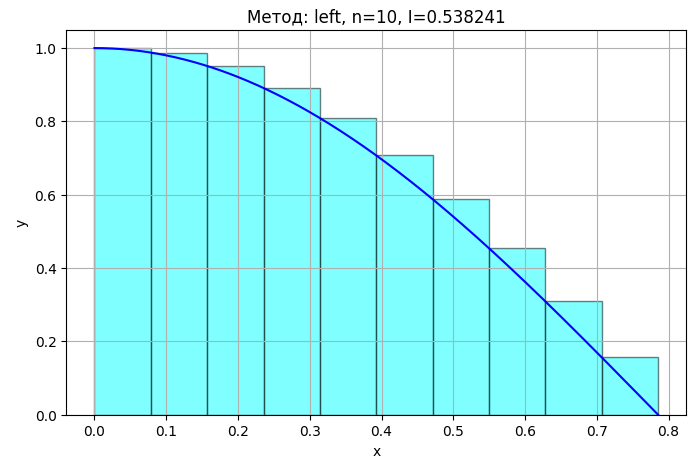
\includegraphics[width=0.6\linewidth]{left_half.png}\\
\(n=10, R = 0.538241\) \\
\(|R_n|\leq \max\limits_{x\in[0,\pi/4]}{|-2\sin{2x}|\frac{(\pi/4)^2}{2n}}=
2\ \cdot\ \frac{(\pi/4)^2}{2n}=\frac{\pi^2}{16n}\) \\
\(|R_n|\leq \frac{\pi^2}{16n}=\frac{\pi^2}{16\cdot 10} \approx 0.061685\)\\
\(|R_n| \leq 0.061685\), \(|R-I|\approx0.038241\),\\
погрешность расчетов не превышает теоретическую.


\newpage

{\large Метод правых прямоугольников}\\
Вычисление ошибки: 
\(|R_n|\leq \max\limits_{x\in[a,b]}{|f'(x)|\frac{(b-a)^2}{2n}}\)\\

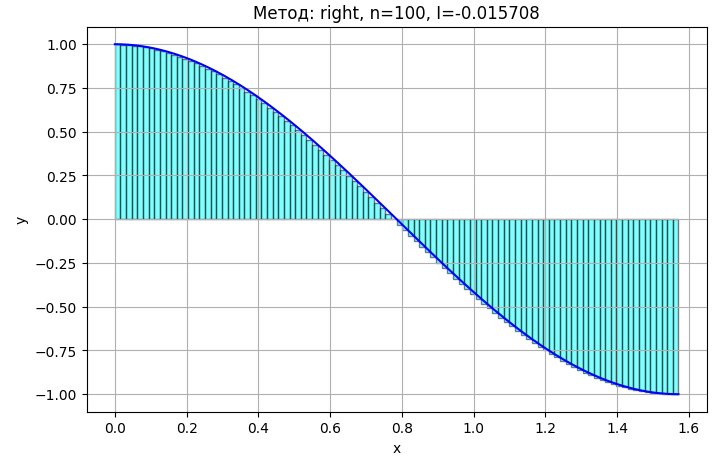
\includegraphics[width=0.6\linewidth]{right_n100.png}\\
\(n=100, R=-0.015708\) \\
\(|R_n|\leq \frac{\pi^2}{4n}=\frac{\pi^2}{4\cdot 100} \approx 0.024674\)\\
\(|R_n| \leq 0.024674\), \(|R-I|\approx0.015708\),\\
погрешность расчетов не превышает теоретическую.

\vspace{0.5cm}

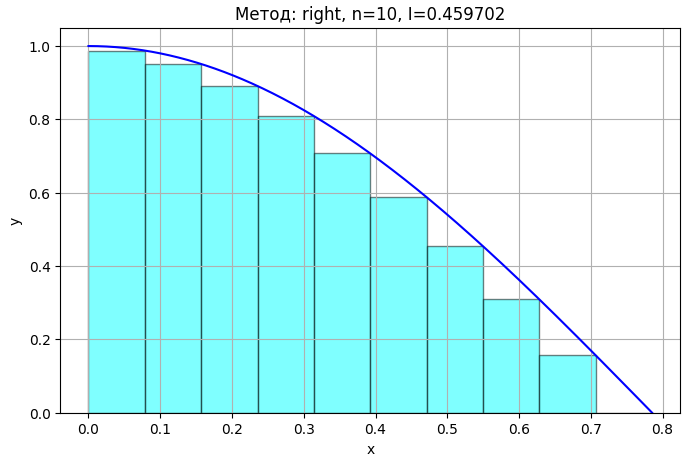
\includegraphics[width=0.6\linewidth]{right_half.png}\\
\(n=10, R=0.459702\) \\
\(|R_n|\leq \frac{\pi^2}{16n}=\frac{\pi^2}{16\cdot 10} \approx 0.061685\)\\
\(|R_n| \leq 0.061685\), \(|R-I|\approx 0.040298\),\\
погрешность расчетов не превышает теоретическую.


\newpage

{\large Метод средних прямоугольников}\\
Вычисление ошибки:
\(|R_n|\leq \max\limits_{x\in[a,b]}{|f''(x)|\frac{(b-a)^3}{24n^2}}\)\\

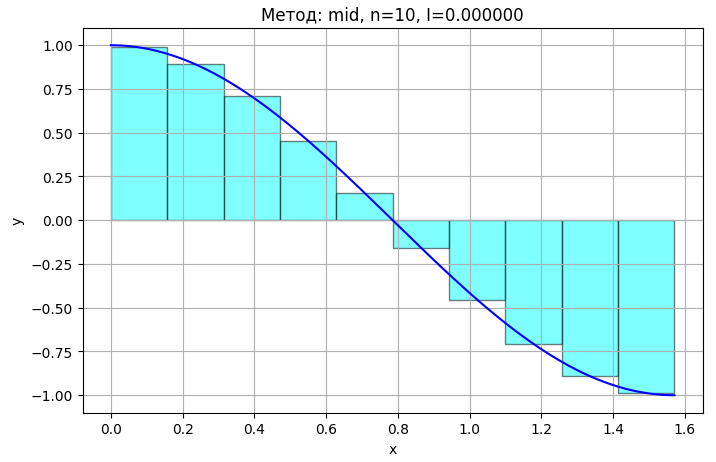
\includegraphics[width=0.6\linewidth]{mid_n10.png}\\
\(n=10, R=0\) \\
\(|R_n| \leq \max\limits_{x\in[0,\pi/2]}{|-4\cos{2x}|\frac{(\pi/2)^3}{24n^2}}=\frac{\pi^3}{48n^2}\)\\
\(|R_n|\leq \frac{\pi^3}{48n^2}=\frac{\pi^3}{48\cdot 100} \approx 0.006459\)
\(|R_n| \leq 0.006459\), \(|R-I| \approx 0\),\\
погрешность расчетов не превышает теоретическую.

\vspace{0.5cm}

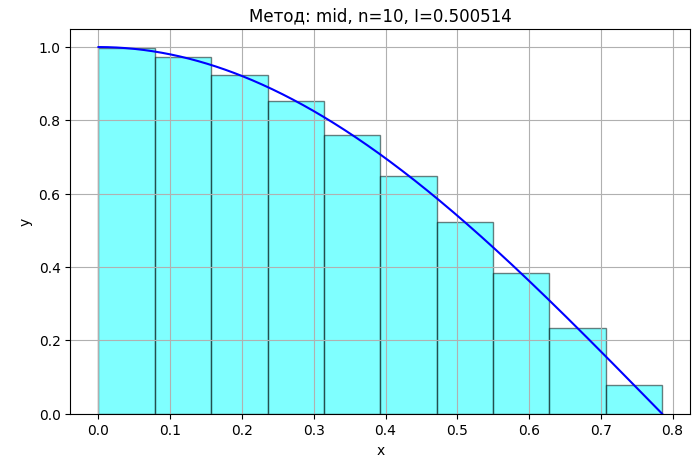
\includegraphics[width=0.6\linewidth]{mid_half.png}\\
\(n=10, R=0.500514\) \\
\(|R_n| \leq \max\limits_{x\in[0,\pi/2]}{|-4\cos{2x}|\frac{(\pi/4)^3}{24n^2}}=\frac{\pi^3}{384n^2}\)\\
\(|R_n|\leq \frac{\pi^3}{384n^2}=\frac{\pi^3}{384\cdot 100} \approx 0.000807\)
\(|R_n| \leq 0.000807\), \(|R-I| \approx 0.000514\),\\
погрешность расчетов не превышает теоретическую.


\newpage

{\large Метод трапеций}\\
Вычисление ошибки: 
\(|R_n|\leq \max\limits_{x\in[a,b]}{|f''(x)|\frac{(b-a)^3}{12n^2}}\)\\

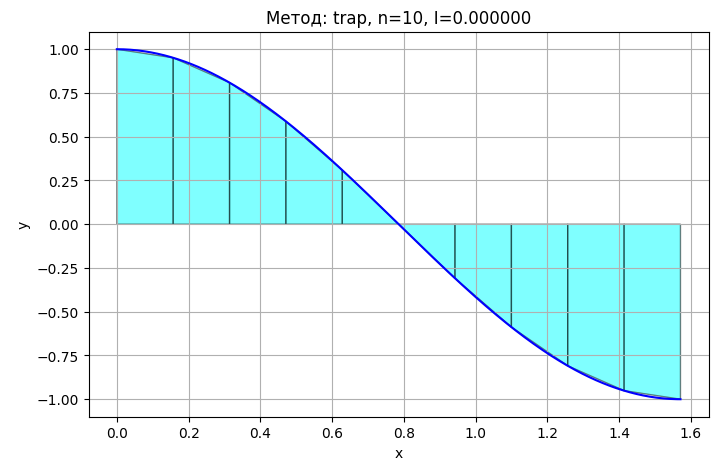
\includegraphics[width=0.7\linewidth]{trap_n10.png}\\
\(n=10, R=0\) \\
\(|R_n| \leq \frac{\pi^3}{24n^2}=\frac{\pi^3}{24\cdot 100} \approx 0.0129192\)
\(|R_n| \leq 0.0129192\), \(|R-I| \approx 0\),\\
погрешность расчетов не превышает теоретическую.

\vspace{0.3cm}

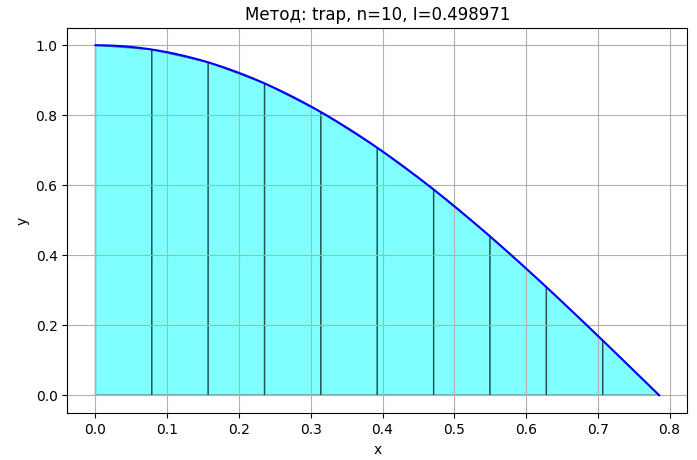
\includegraphics[width=0.7\linewidth]{trap_half.png}\\
\(n=10, R=0.498971\) \\
\(|R_n| \leq \frac{\pi^3}{192n^2}=\frac{\pi^3}{192\cdot 100} \approx 0.001614\)
\(|R_n| \leq 0.001614\), \(|R-I| \approx 0.001029\),\\
погрешность расчетов не превышает теоретическую.

Отметим, что \(\cos{2x} \in C^2[0, \pi/2]\), так что все полученные оценки погрешности корректны. Для всех четырех методов выполняется:\\ \(|R_n| \xrightarrow{n \to \infty}{} 0\).

\end{document}

